\documentclass[aspectratio=169]{beamer}
%\documentclass[handout]{beamer}

% language settings
%\usepackage{fontspec, polyglossia}
%\setdefaultlanguage{magyar}

% common packages
\usepackage{amsmath, multimedia, hyperref, color, multirow}
%\usepackage{graphicx}
\usepackage{pifont}

% TikZ
\usepackage{tikz}
\usetikzlibrary{arrows.meta, decorations.pathmorphing, decorations.pathreplacing, shapes.geometric,mindmap}
\usetikzlibrary{shapes.geometric,fadings,bayesnet}

% beamer styles
\mode<presentation>{
%\usetheme{Pittsburgh}
\usetheme{Antibes}
\usecolortheme{beaver}
%\usecolortheme{seahorse}
%\usefonttheme{structureitalicserif}
\setbeamercovered{transparent}
}
\setbeamertemplate{blocks}[rounded][shadow=true]
\AtBeginSubsection[]{
  \begin{frame}<beamer>{Contents}
  \end{frame}
}
%\useoutertheme[]{tree}

% title, etc
%\title{Drug Repurposing to Alzheimer's Disease Using TWAS and the PPI Network}
\title{Network Based Drug Repurposing to Alzheimer's}
\author{Attila Jones}
\date{CTNS: Clinical \& Translational Neuroscience Section}

\begin{document}

\maketitle

\begin{frame}{DREAM}{Drug Repurposing for Effective Alzheimer's Medicines}
\begin{columns}[t]
\begin{column}{0.4\textwidth}
\begin{enumerate}
\item<1-> AD risk genes
\begin{itemize}
\item<1> curated knowledge
\item<2> our AD gene discoveries
\item<3> public omic data
\end{itemize}
\item<4-> prioritize approved drugs
\begin{itemize}
\item<4> network based proximity
\end{itemize}
\item<5-> validate
\begin{itemize}
\item \emph{in vitro} essays
\item pharmacoepidemiology
\end{itemize}
\end{enumerate}
\end{column}

\begin{column}{0.6\textwidth}

\includegraphics<1>[width=0.3\columnwidth]{figures/from-others/uniprot-logo.png}
\includegraphics<1>[width=0.3\columnwidth]{figures/from-others/amyco-logo.png}

\includegraphics<2>[width=0.8\columnwidth]{figures/from-others/jackson-APOE-Fig2c.png}

\only<2>{\tiny Roberts,..., Thambisetty 2021 Science Advances}

\includegraphics<3>[width=1.0\columnwidth]{figures/from-others/schwartzentruber-fig1b.png}

\only<3>{\tiny Schwartzentruber et al 2021 Nat Genet}

\includegraphics<4>[width=0.3\columnwidth]{figures/from-others/drugbank-logo.png}

\includegraphics<4>[width=0.5\columnwidth]{figures/from-others/rual-2005-interactome-Fig2b.png}

%\includegraphics<3>[width=0.2\columnwidth]{figures/from-others/gtex.png}
\end{column}
\end{columns}
\end{frame}

\begin{frame}{Approaches to drug repurposing}
\begin{columns}[t]
\begin{column}{0.6\textwidth}

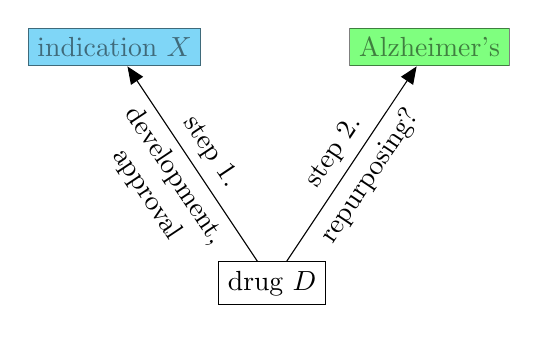
\begin{tikzpicture}
\path (0,0) node[draw] (drug) {drug $D$}
	(-2,3) node[draw,fill=cyan,semitransparent] (ind) {indication $X$}
	( 2,3) node[draw,fill=green,semitransparent] (alz) {Alzheimer's};
\path[->] (drug) edge node[below,sloped,text width=3cm,text centered] {development, approval} node[above,sloped]
	{step 1.} (ind);
\path[->] (drug) edge node[below,sloped] {repurposing?} node[above,sloped]
	{step 2.} (alz);
\end{tikzpicture}
\end{column}

\begin{column}{0.4\textwidth}
\begin{enumerate}
\item shared gene approach\\
	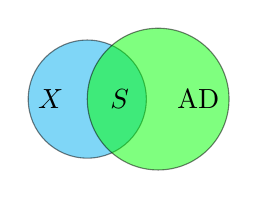
\begin{tikzpicture}[scale=1.5]
\draw[fill=cyan,semitransparent] (0,0) circle (0.5cm);
\draw[fill=green,semitransparent] (0.6,0) circle (0.6cm);
\draw (0.275cm,0) node {$S$};
\draw (1.2cm,0) node[anchor=east] {AD};
%\draw (0.6cm,0.6) node[anchor=south] {AD};
\draw (-0.5cm,0.0) node[anchor=west] {$X$};
\end{tikzpicture}

%\footnotesize
%shared genes $S = X \cap \mathrm{AD}$
\normalsize
\item network based appr.
\begin{description}
\footnotesize
\item[Guney,..., Barabási 2016] proximity
\item[Cheng,..., Barabási 2018] validation
\end{description}
\end{enumerate}
\end{column}
\end{columns}
\end{frame}

\begin{frame}{Network based proximity}
\begin{equation*}
	d = \frac{1}{|T|}\sum_{t \in T} \min_{s \in S} d(s, t),
\end{equation*}
\end{frame}

\end{document}
